%%%%%%%%%%%%%%%%%%%%%%%%%%%%%%%%%%%%%%%%%%%%%%%%%%%%%%%%%%%%%%%%%%%%%%%%%%%%%%%%%%
\begin{frame}[fragile]\frametitle{}
\begin{center}
{\Large LLM in Production}

{\tiny (Ref: MLOps.community channel on Youtube)}

\end{center}
\end{frame}

%%%%%%%%%%%%%%%%%%%%%%%%%%%%%%%%%%%%%%%%%%%%%%%%%%%%%%%%%%%
\begin{frame}[fragile]\frametitle{Compare before use}

\begin{center}
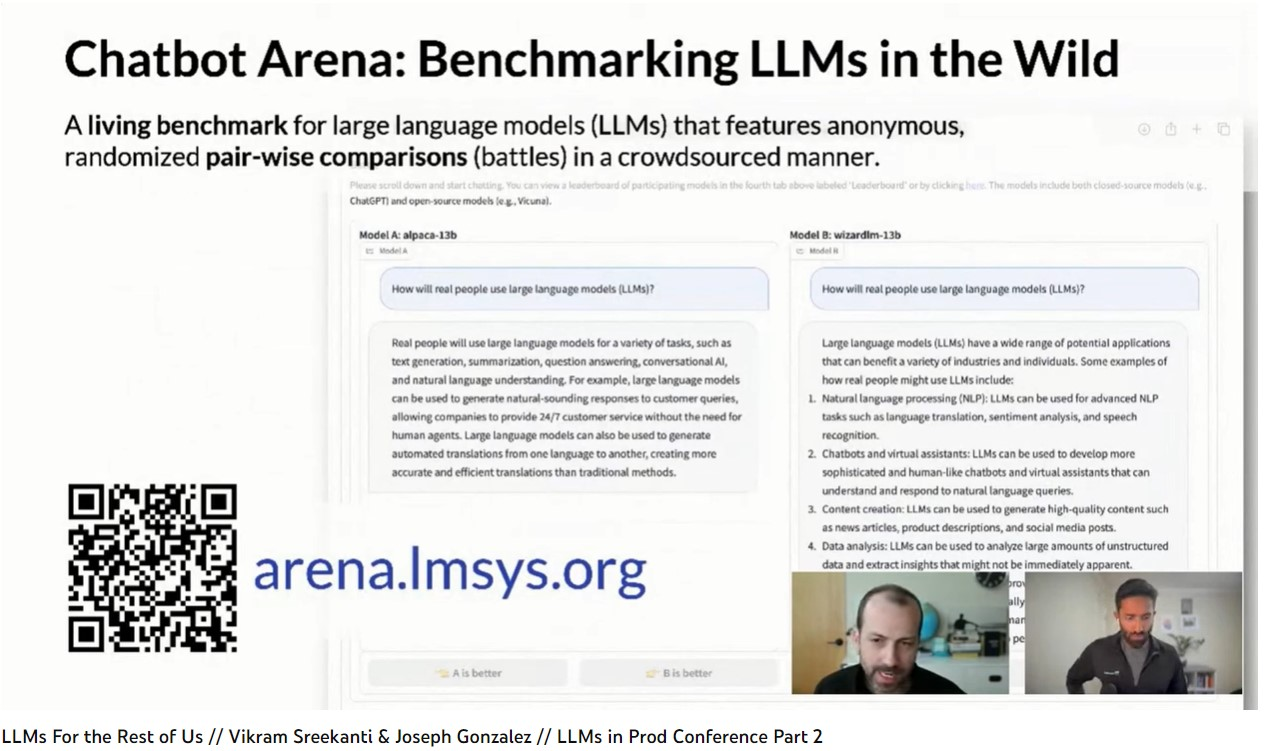
\includegraphics[width=\linewidth,keepaspectratio]{llm57}
\end{center}
\end{frame}

%%%%%%%%%%%%%%%%%%%%%%%%%%%%%%%%%%%%%%%%%%%%%%%%%%%%%%%%%%%
\begin{frame}[fragile]\frametitle{Missing Link}
\begin{columns}
    \begin{column}[T]{0.5\linewidth}
		\begin{itemize}
		\item Good models are hosted ones, so you tend to build own (foundation) model, do you really need it? Use largest that you can afford/use.
		\item Use your own data via Vector Databases
		\item Exhausting prompt engineering, chaining, orchestration frameworks.
		\item Be specific and not expect that models will do everything.
		\item Have good data quality and governance and also good Validation, tracing and logging.
		\end{itemize}	
    \end{column}
    \begin{column}[T]{0.5\linewidth}
		\begin{center}
			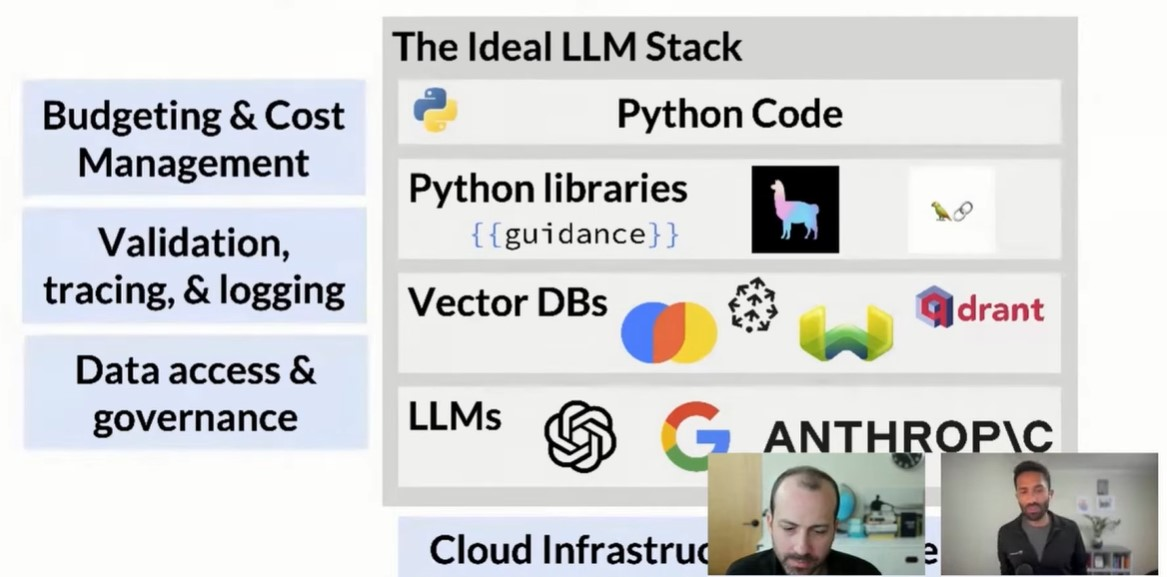
\includegraphics[width=\linewidth,keepaspectratio]{llm58}
		\end{center}
	\end{column}
  \end{columns}
\end{frame}


%%%%%%%%%%%%%%%%%%%%%%%%%%%%%%%%%%%%%%%%%%%%%%%%%%%%%%%%%%%
\begin{frame}[fragile]\frametitle{Customizing Solutions}

\begin{itemize}
\item Fine tuning: few shots, whole model
\item Hand crafted prompts
\item Optimization
	\begin{itemize}
	\item Programmatic prompt generation (human readable)
	\item AutoPrompt (Gradient based searches), not human readable
	\item Continuous: P-tuning, Prefix-tuning
	\end{itemize}
\item RLHF (Reinforcement Learning with Human Feedback)
\end{itemize}	

Which one is most appropriate? What about platforms which provide customization?
\end{frame}


%%%%%%%%%%%%%%%%%%%%%%%%%%%%%%%%%%%%%%%%%%%%%%%%%%%%%%%%%%%
\begin{frame}[fragile]\frametitle{Evaluation}

\begin{itemize}
\item `Hero` use cases ( say smoke test, must work)
\item White box testing
\item Edge cases, missing conflicting data
\item User feedback, bugs
\item Out of scope functionality, graceful denial.
\end{itemize}

{\tiny (Ref: Combining LLMs with Knowledge Bases to Prevent Hallucinations - Scott Mackie - LLMs in Prod Con 2 )}

\end{frame}

%%%%%%%%%%%%%%%%%%%%%%%%%%%%%%%%%%%%%%%%%%%%%%%%%%%%%%%%%%%
\begin{frame}[fragile]\frametitle{How to Evaluate}

\begin{itemize}
\item We don't have test-train distribution used during training, as we did not do the trainin itself. So there is always a DRIFT.
\item Evaluation is qualitative than quantitative.
\item Trained on ALL subjects but being used for ONE/TWO domains, hard to measure then.
\end{itemize}

\begin{center}
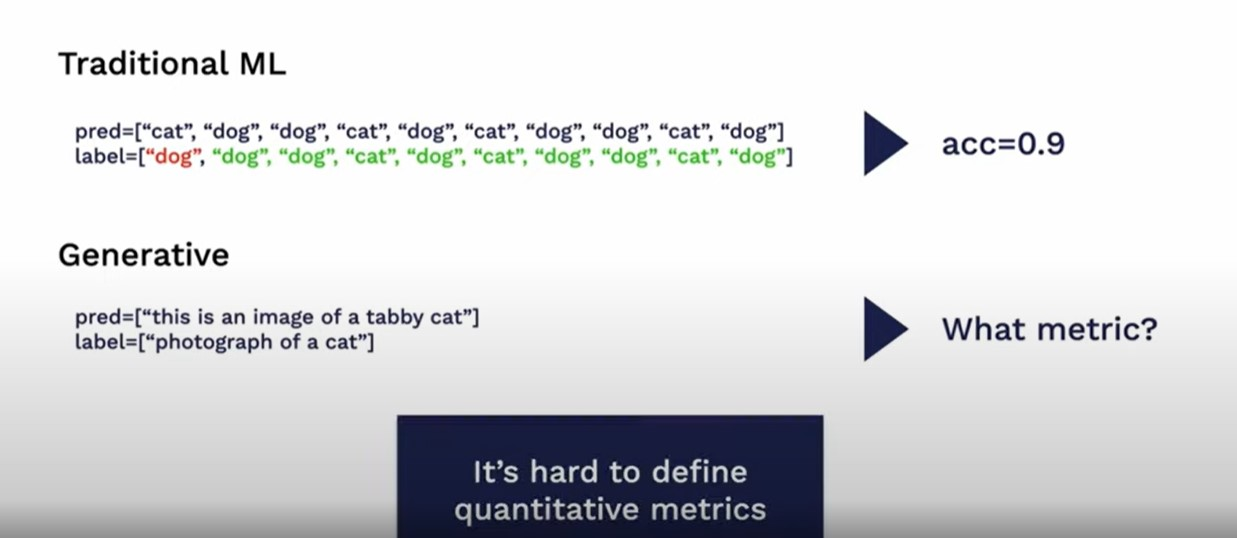
\includegraphics[width=0.6\linewidth,keepaspectratio]{llm68}
\end{center}		


{\tiny (Ref: Evaluating LLM-based Applications // Josh Tobin // LLMs in Prod Conference Part 2 )}

\end{frame}

%%%%%%%%%%%%%%%%%%%%%%%%%%%%%%%%%%%%%%%%%%%%%%%%%%%%%%%%%%%
\begin{frame}[fragile]\frametitle{How much it costs to Evaluate}

\begin{itemize}
\item We don't have test-train distribution used during training, as we did not do the trainin itself. So there is always a DRIFT.
\item Evaluation is qualitative than quantitative.
\item Trained on ALL subjects but being used for ONE/TWO domains, hard to measure then.
\end{itemize}

\begin{center}
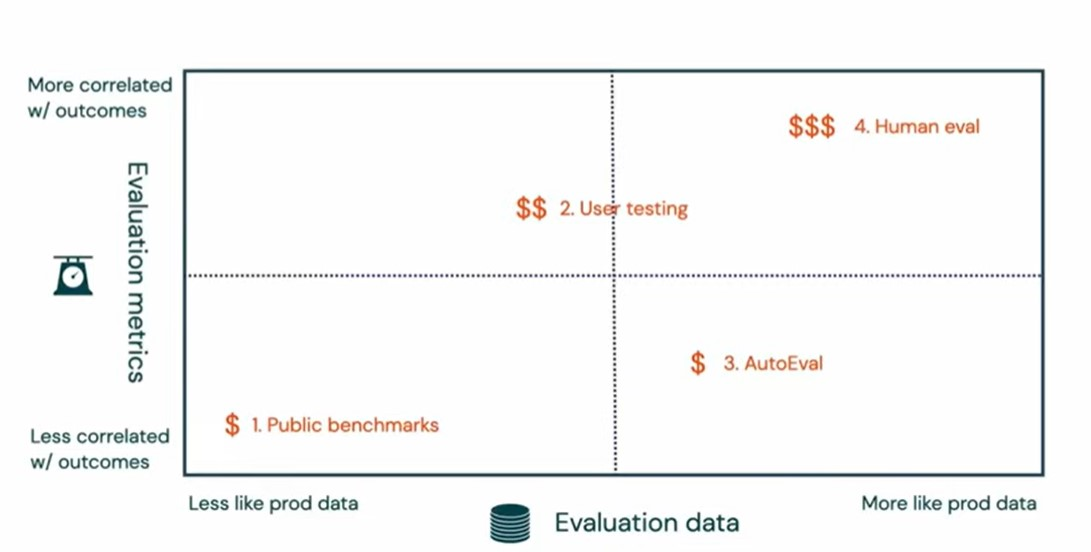
\includegraphics[width=0.8\linewidth,keepaspectratio]{llm69}
\end{center}		


{\tiny (Ref: Evaluating LLM-based Applications // Josh Tobin // LLMs in Prod Conference Part 2 )}

\end{frame}

%%%%%%%%%%%%%%%%%%%%%%%%%%%%%%%%%%%%%%%%%%%%%%%%%%%%%%%%%%%
\begin{frame}[fragile]\frametitle{How to Evaluate}

\begin{itemize}
\item Functional correctness: Code generation models are easy to check
\item Model evaluation models are getting popular.
\item BLUE is getting out of favor due to biases.
\end{itemize}

\begin{center}
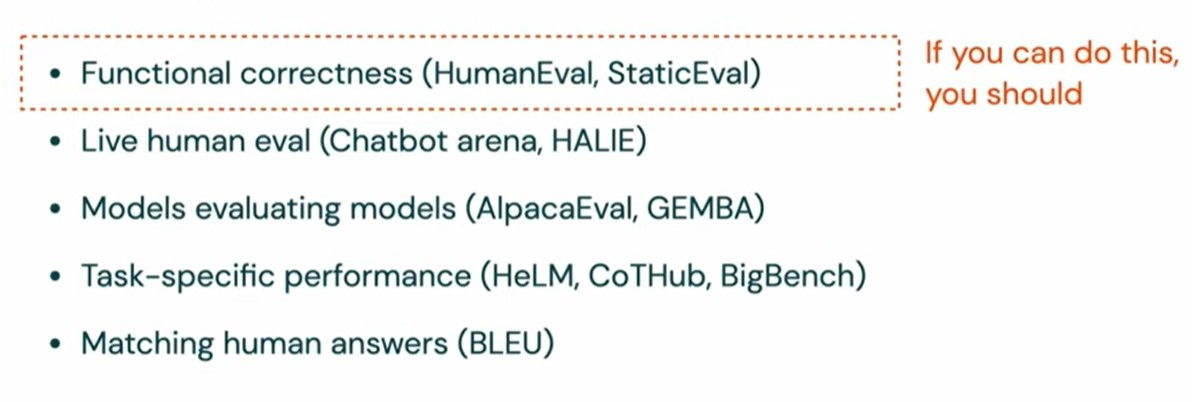
\includegraphics[width=0.8\linewidth,keepaspectratio]{llm70}
\end{center}		


{\tiny (Ref: Evaluating LLM-based Applications // Josh Tobin // LLMs in Prod Conference Part 2 )}

\end{frame}

%%%%%%%%%%%%%%%%%%%%%%%%%%%%%%%%%%%%%%%%%%%%%%%%%%%%%%%%%%%
\begin{frame}[fragile]\frametitle{How to Evaluate}


\begin{center}
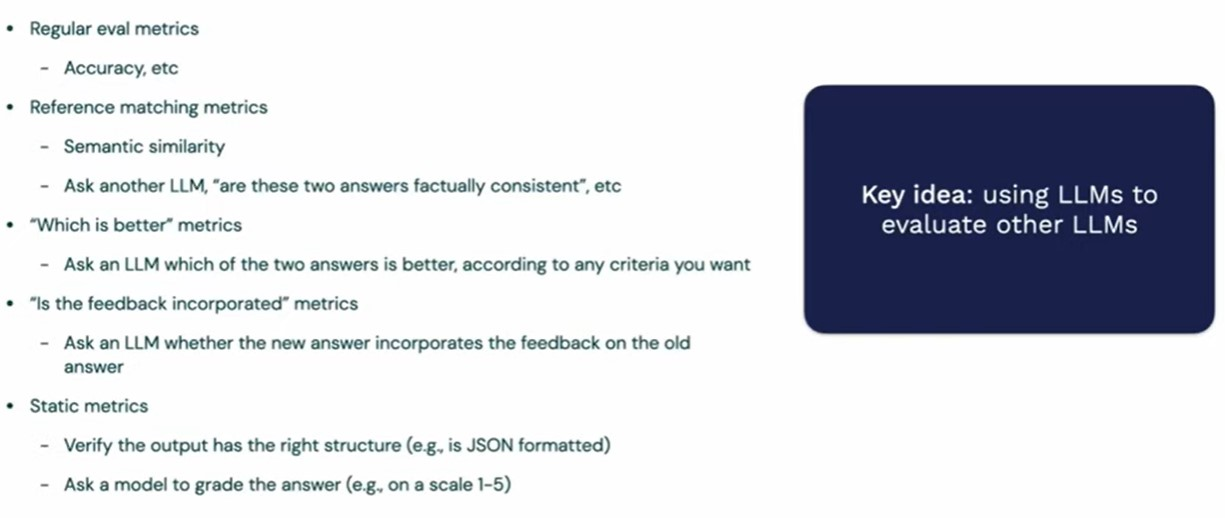
\includegraphics[width=0.8\linewidth,keepaspectratio]{llm71}
\end{center}		

Just note than as LLMs can be biased, using them for evaluation can be limiting. Watching the Watchman!!
Last resort is of course High Quality Human Evaluation.

{\tiny (Ref: Evaluating LLM-based Applications // Josh Tobin // LLMs in Prod Conference Part 2 )}

\end{frame}

%%%%%%%%%%%%%%%%%%%%%%%%%%%%%%%%%%%%%%%%%%%%%%%%%%%%%%%%%%%
\begin{frame}[fragile]\frametitle{How to do costing}

Problem statement: 50\% summarization of whole Wikipedia

\begin{center}
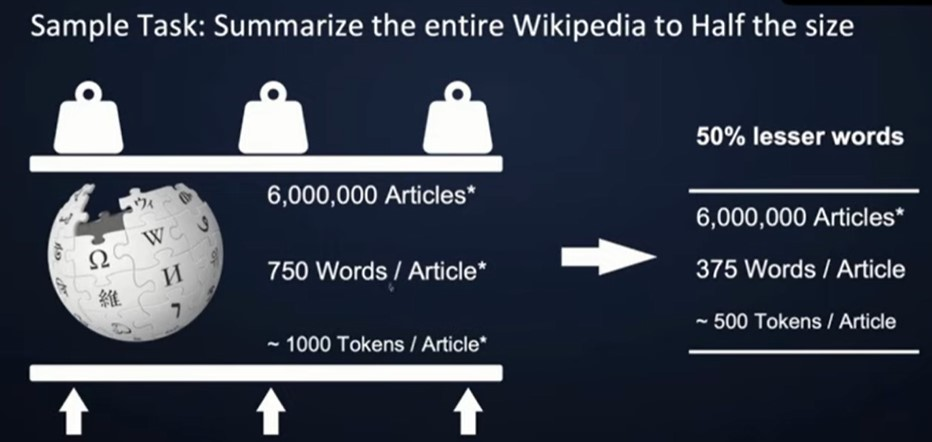
\includegraphics[width=0.8\linewidth,keepaspectratio]{llm72}
\end{center}		



{\tiny (Ref: \$360k Question - Understanding the LLM Economics // Nikunj Bajaj // LLMs in Production Conference )}

\end{frame}

%%%%%%%%%%%%%%%%%%%%%%%%%%%%%%%%%%%%%%%%%%%%%%%%%%%%%%%%%%%
\begin{frame}[fragile]\frametitle{How to do costing}


\begin{center}
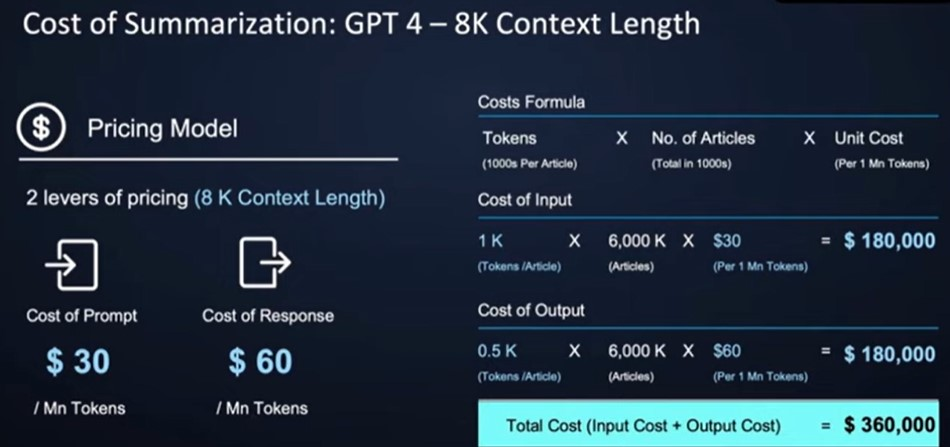
\includegraphics[width=0.8\linewidth,keepaspectratio]{llm73}
\end{center}		



{\tiny (Ref: \$360k Question - Understanding the LLM Economics // Nikunj Bajaj // LLMs in Production Conference )}

\end{frame}

%%%%%%%%%%%%%%%%%%%%%%%%%%%%%%%%%%%%%%%%%%%%%%%%%%%%%%%%%%%
\begin{frame}[fragile]\frametitle{How to do costing}

If we choose bigger context length

\begin{center}
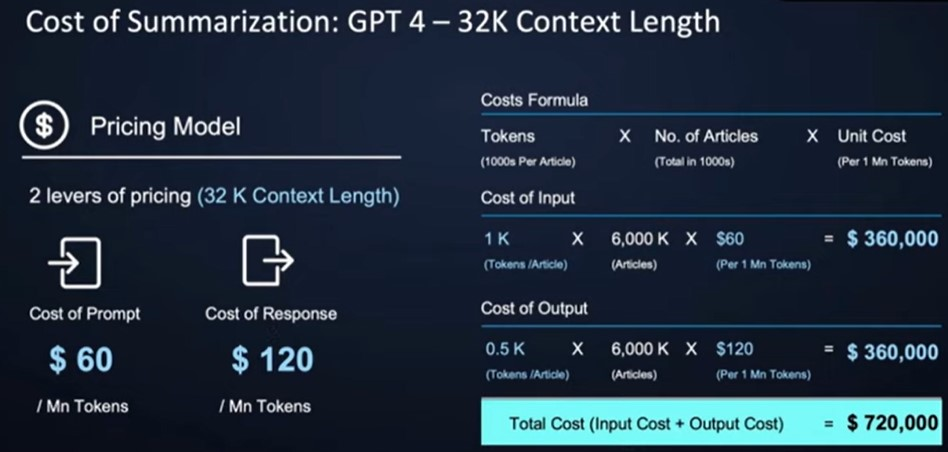
\includegraphics[width=0.8\linewidth,keepaspectratio]{llm74}
\end{center}		



{\tiny (Ref: \$360k Question - Understanding the LLM Economics // Nikunj Bajaj // LLMs in Production Conference )}

\end{frame}

%%%%%%%%%%%%%%%%%%%%%%%%%%%%%%%%%%%%%%%%%%%%%%%%%%%%%%%%%%%
\begin{frame}[fragile]\frametitle{How to do costing}

With Da Vinci

\begin{center}
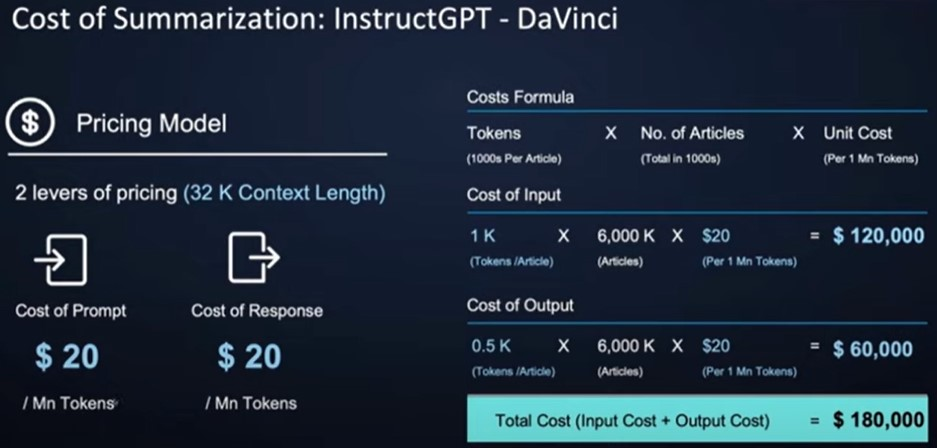
\includegraphics[width=0.8\linewidth,keepaspectratio]{llm75}
\end{center}		



{\tiny (Ref: \$360k Question - Understanding the LLM Economics // Nikunj Bajaj // LLMs in Production Conference )}

\end{frame}

%%%%%%%%%%%%%%%%%%%%%%%%%%%%%%%%%%%%%%%%%%%%%%%%%%%%%%%%%%%
\begin{frame}[fragile]\frametitle{How to do costing}

With Curie

\begin{center}
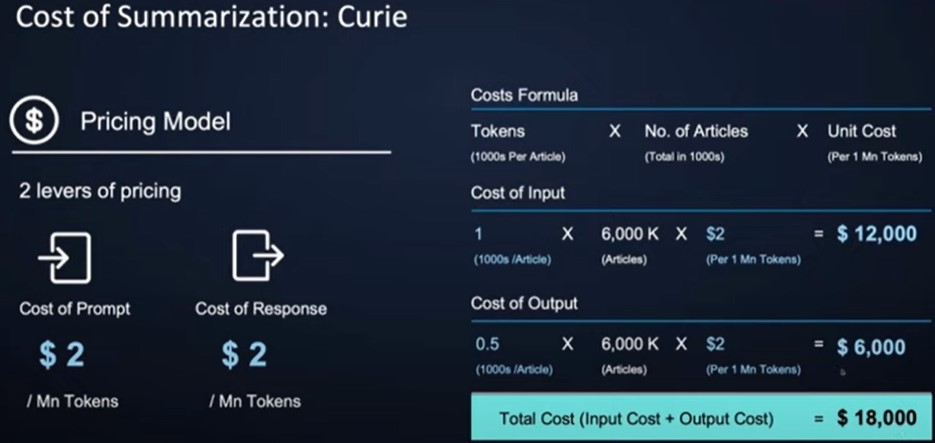
\includegraphics[width=0.8\linewidth,keepaspectratio]{llm76}
\end{center}		



{\tiny (Ref: \$360k Question - Understanding the LLM Economics // Nikunj Bajaj // LLMs in Production Conference )}

\end{frame}

%%%%%%%%%%%%%%%%%%%%%%%%%%%%%%%%%%%%%%%%%%%%%%%%%%%%%%%%%%%
\begin{frame}[fragile]\frametitle{How to do costing}

With self hosted model, speed is assumed to be n tokens per hour

\begin{center}
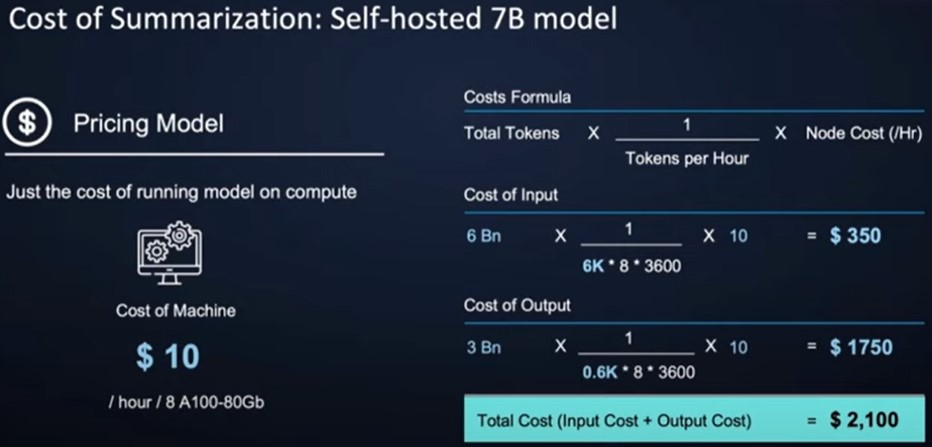
\includegraphics[width=0.8\linewidth,keepaspectratio]{llm77}
\end{center}		



{\tiny (Ref: \$360k Question - Understanding the LLM Economics // Nikunj Bajaj // LLMs in Production Conference )}

\end{frame}

%%%%%%%%%%%%%%%%%%%%%%%%%%%%%%%%%%%%%%%%%%%%%%%%%%%%%%%%%%%
\begin{frame}[fragile]\frametitle{How to do costing}

Fine tuning (Da vinci 1.2M, Curie 126k)
\begin{center}
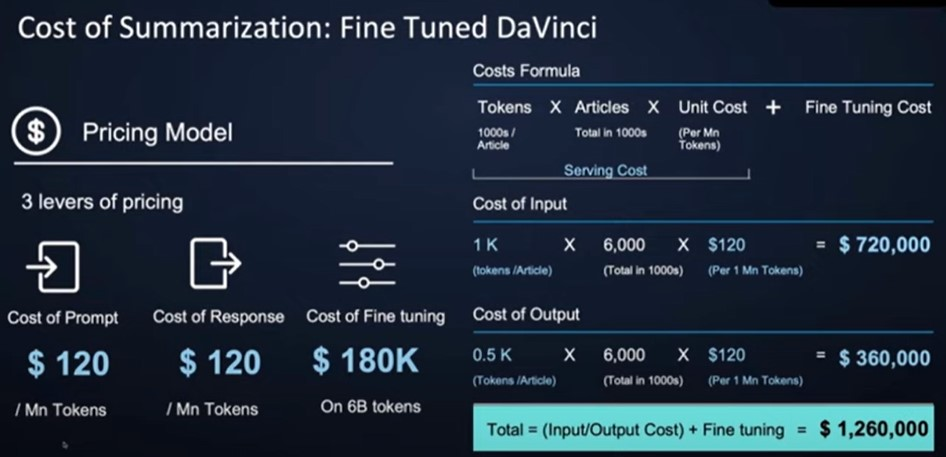
\includegraphics[width=0.8\linewidth,keepaspectratio]{llm78}
\end{center}		



{\tiny (Ref: \$360k Question - Understanding the LLM Economics // Nikunj Bajaj // LLMs in Production Conference )}

\end{frame}

%%%%%%%%%%%%%%%%%%%%%%%%%%%%%%%%%%%%%%%%%%%%%%%%%%%%%%%%%%%
\begin{frame}[fragile]\frametitle{How to do costing}

Fine tuning Self Hosted
\begin{center}
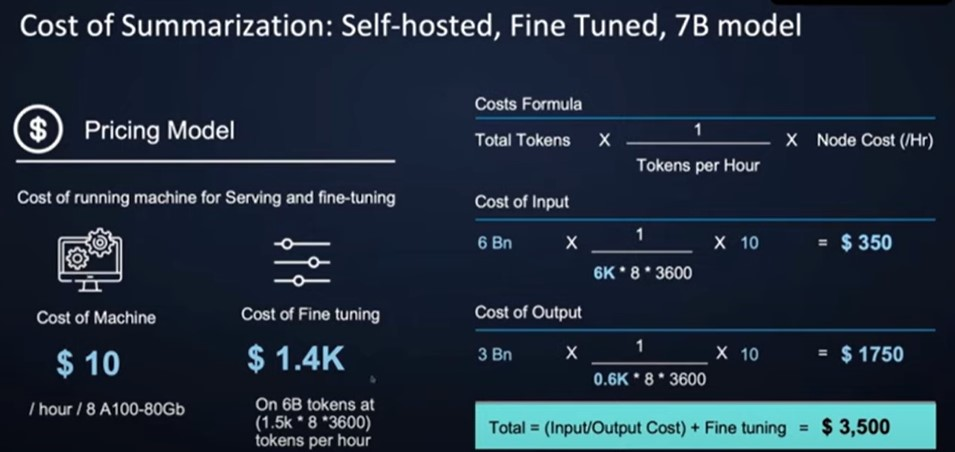
\includegraphics[width=0.8\linewidth,keepaspectratio]{llm79}
\end{center}		



{\tiny (Ref: \$360k Question - Understanding the LLM Economics // Nikunj Bajaj // LLMs in Production Conference )}

\end{frame}

%%%%%%%%%%%%%%%%%%%%%%%%%%%%%%%%%%%%%%%%%%%%%%%%%%%%%%%%%%%
\begin{frame}[fragile]\frametitle{How to do costing}

Summary 

\begin{center}
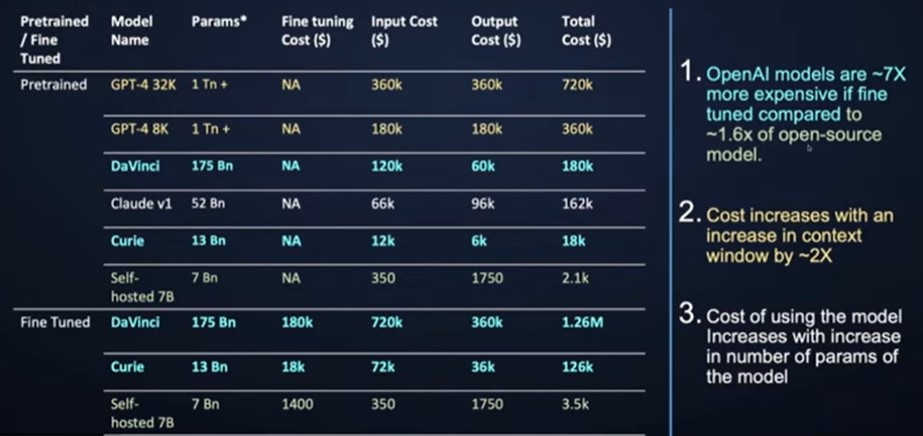
\includegraphics[width=0.8\linewidth,keepaspectratio]{llm80}
\end{center}		



{\tiny (Ref: \$360k Question - Understanding the LLM Economics // Nikunj Bajaj // LLMs in Production Conference )}

\end{frame}

%%%%%%%%%%%%%%%%%%%%%%%%%%%%%%%%%%%%%%%%%%%%%%%%%%%%%%%%%%%
\begin{frame}[fragile]\frametitle{How to do costing}

Summary with quality also

\begin{center}
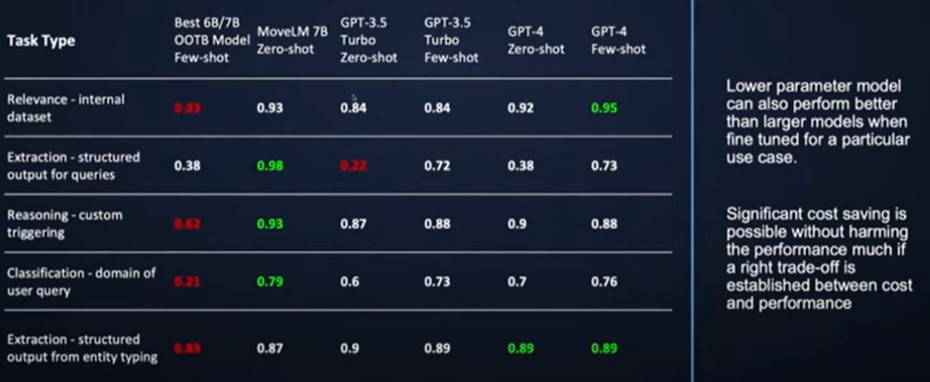
\includegraphics[width=0.8\linewidth,keepaspectratio]{llm81}
\end{center}		

Open source LLM with fine tuning is the recommendation.


{\tiny (Ref: \$360k Question - Understanding the LLM Economics // Nikunj Bajaj // LLMs in Production Conference )}

\end{frame}




%%%%%%%%%%%%%%%%%%%%%%%%%%%%%%%%%%%%%%%%%%%%%%%%%%%%%%%%%%%
\begin{frame}[fragile]\frametitle{Shared Responsibility Model}

\begin{center}
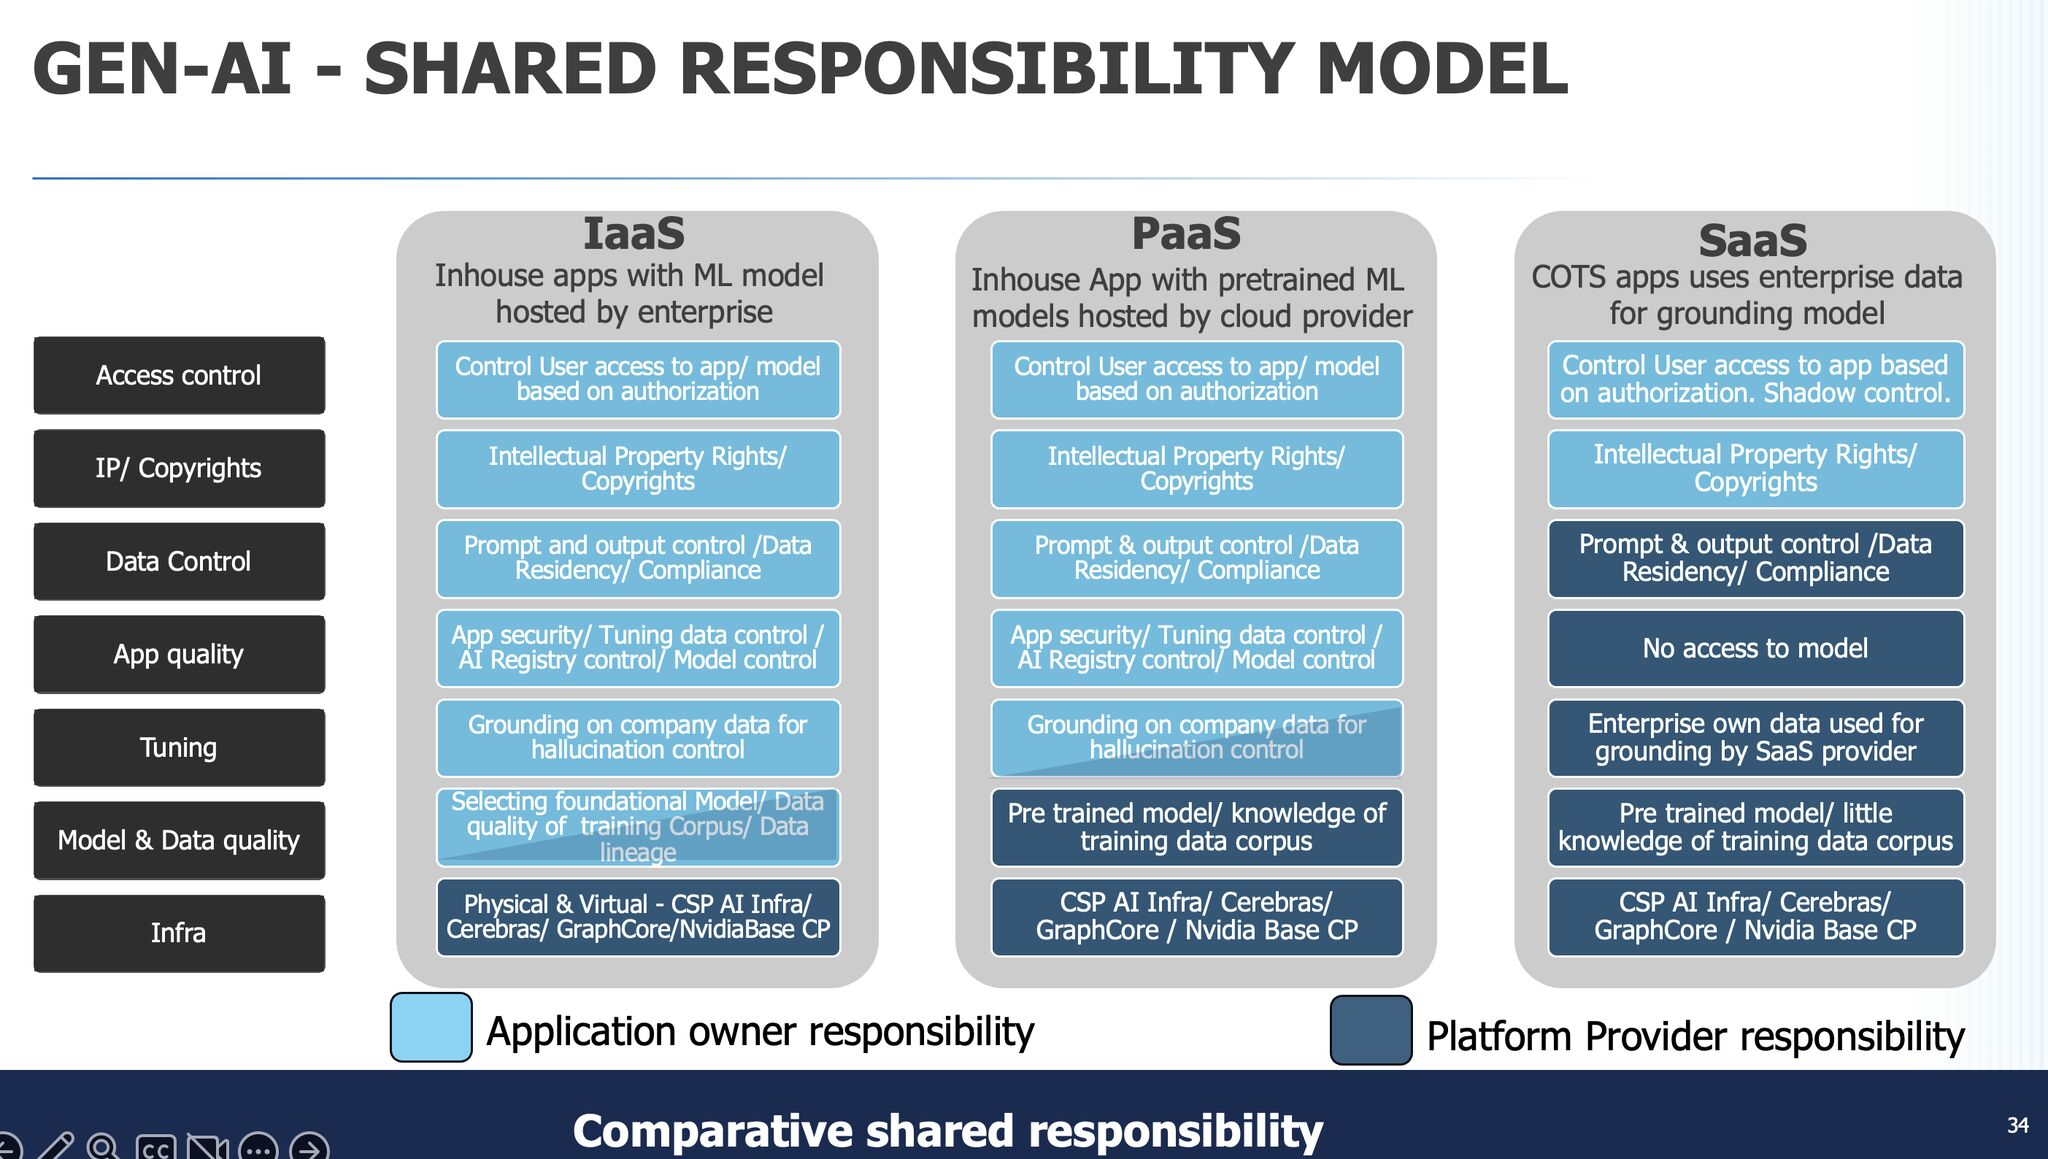
\includegraphics[width=\linewidth,keepaspectratio]{llm63}
\end{center}		


{\tiny (Ref: Linkedin Post on 11 Aug 2023 by - Vishwas Manral )}

\end{frame}


%%%%%%%%%%%%%%%%%%%%%%%%%%%%%%%%%%%%%%%%%%%%%%%%%%%%%%%%%%%
\begin{frame}[fragile]\frametitle{Commercial Example: Intuit GenOS}

\begin{itemize}
    \item GenStudio: Dev environment for rapid experimentation with generative AI experiences.
    \item GenRuntime: Intelligent layer choosing appropriate large language model in real time, based on user needs.
    \item GenUX: Library of UI components and user flows for clear and delightful interactions.
    \item Financial LLMs: Custom trained for tax, accounting, marketing, etc., providing insights and actions.
\end{itemize}

\end{frame}

%%%%%%%%%%%%%%%%%%%%%%%%%%%%%%%%%%%%%%%%%%%%%%%%%%%%%%%%%%%%%%%%%%%%%%%%%%%%%%%%%%
\begin{frame}[fragile]\frametitle{Challenges of Building LLM App}


\begin{center}
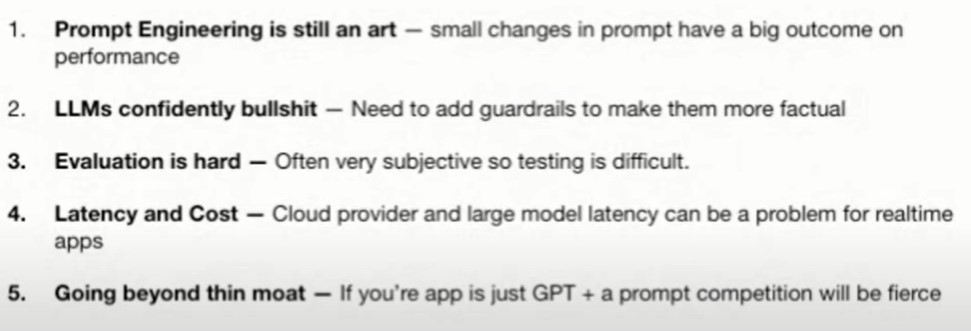
\includegraphics[width=0.7\linewidth,keepaspectratio]{llm83}

\end{center}

{\tiny (Ref: Pitfalls and Best Practices — 5 lessons from LLMs in Production // Raza Habib // LLMs in Prod Con 2)}
\end{frame}

%%%%%%%%%%%%%%%%%%%%%%%%%%%%%%%%%%%%%%%%%%%%%%%%%%%%%%%%%%%%%%%%%%%%%%%%%%%%%%%%%%
\begin{frame}[fragile]\frametitle{Challenges of Building LLM App}


\begin{center}
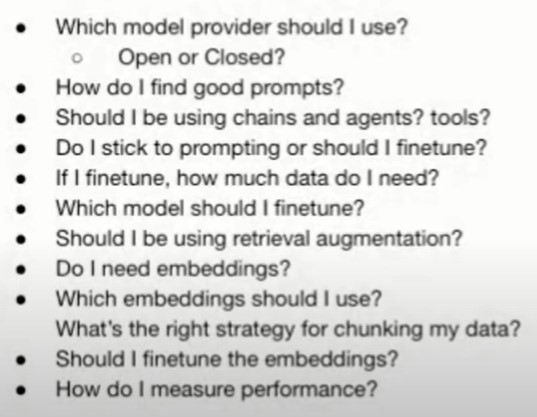
\includegraphics[width=0.7\linewidth,keepaspectratio]{llm84}

\end{center}

{\tiny (Ref: Pitfalls and Best Practices — 5 lessons from LLMs in Production // Raza Habib // LLMs in Prod Con 2)}
\end{frame}


